%%%%%%%%%%%%%%%%%%%%%%%%%%%%%%%%%%%%%%%%%%%%%%%%%%%%%%%%%%%%%%%%%%%%%%
%%  Copyright by Wenliang Du.                                       %%
%%  This work is licensed under the Creative Commons                %%
%%  Attribution-NonCommercial-ShareAlike 4.0 International License. %%
%%  To view a copy of this license, visit                           %%
%%  http://creativecommons.org/licenses/by-nc-sa/4.0/.              %%
%%%%%%%%%%%%%%%%%%%%%%%%%%%%%%%%%%%%%%%%%%%%%%%%%%%%%%%%%%%%%%%%%%%%%%

\newcommand{\commonfolder}{../../common-files}

\documentclass[11pt]{article}

\usepackage[most]{tcolorbox}
\usepackage{times}
\usepackage{epsf}
\usepackage{epsfig}
\usepackage{amsmath, alltt, amssymb, xspace}
\usepackage{wrapfig}
\usepackage{fancyhdr}
\usepackage{url}
\usepackage{verbatim}
\usepackage{fancyvrb}
\usepackage{adjustbox}
\usepackage{listings}
\usepackage{color}
\usepackage{subfigure}
\usepackage{cite}
\usepackage{sidecap}
\usepackage{pifont}
\usepackage{mdframed}
\usepackage{textcomp}
\usepackage{enumitem}
\usepackage{hyperref}


% Horizontal alignment
\topmargin      -0.50in  % distance to headers
\oddsidemargin  0.0in
\evensidemargin 0.0in
\textwidth      6.5in
\textheight     8.9in 

\newcommand{\todo}[1]{
\vspace{0.1in}
\fbox{\parbox{6in}{TODO: #1}}
\vspace{0.1in}
}


\newcommand{\unix}{{\tt Unix}\xspace}
\newcommand{\linux}{{\tt Linux}\xspace}
\newcommand{\minix}{{\tt Minix}\xspace}
\newcommand{\ubuntu}{{\tt Ubuntu}\xspace}
\newcommand{\setuid}{{\tt Set-UID}\xspace}
\newcommand{\openssl} {\texttt{openssl}}


\pagestyle{fancy}
\lhead{\bfseries SEED Labs}
\chead{}
\rhead{\small \thepage}
\lfoot{}
\cfoot{}
\rfoot{}


\definecolor{dkgreen}{rgb}{0,0.6,0}
\definecolor{gray}{rgb}{0.5,0.5,0.5}
\definecolor{mauve}{rgb}{0.58,0,0.82}
\definecolor{lightgray}{gray}{0.90}


\lstset{%
  frame=none,
  language=,
  backgroundcolor=\color{lightgray},
  aboveskip=3mm,
  belowskip=3mm,
  showstringspaces=false,
%  columns=flexible,
  basicstyle={\small\ttfamily},
  numbers=none,
  numberstyle=\tiny\color{gray},
  keywordstyle=\color{blue},
  commentstyle=\color{dkgreen},
  stringstyle=\color{mauve},
  breaklines=true,
  breakatwhitespace=true,
  tabsize=3,
  columns=fullflexible,
  keepspaces=true,
  escapeinside={(*@}{@*)}
}

\newcommand{\newnote}[1]{
\vspace{0.1in}
\noindent
\fbox{\parbox{1.0\textwidth}{\textbf{Note:} #1}}
%\vspace{0.1in}
}


%% Submission
\newcommand{\seedsubmission}{
Debe enviar un informe de laboratorio detallado, con capturas de pantalla, para describir lo que ha hecho y lo que ha observado.
También debe proporcionar una explicación a las observaciones que sean interesantes o sorprendentes.
Enumere también los fragmentos de código más importantes seguidos de una explicación. No recibirán créditos aquellos fragmentos de códigos que no sean explicados.}

%% Book
\newcommand{\seedbook}{\textit{Computer \& Internet Security: A Hands-on Approach}, 2nd
Edition, by Wenliang Du. Para más detalles \url{https://www.handsonsecurity.net}.\xspace}

%% Videos
\newcommand{\seedisvideo}{\textit{Internet Security: A Hands-on Approach},
by Wenliang Du. Para más detalles \url{https://www.handsonsecurity.net/video.html}.\xspace}

\newcommand{\seedcsvideo}{\textit{Computer Security: A Hands-on Approach},
by Wenliang Du. Para más detalles \url{https://www.handsonsecurity.net/video.html}.\xspace}

%% Lab Environment
\newcommand{\seedenvironment}{Este laboratorio ha sido testeado en nuestra imagen pre-compilada de una VM con Ubuntu 16.04, que puede ser descargada del sitio oficial de SEED.\xspace}

\newcommand{\seedenvironmentA}{Este laboratorio ha sido testeado en nuestra imagen pre-compilada de una VM con Ubuntu 16.04, que puede ser descargada del sitio oficial de SEED.\xspace}

\newcommand{\seedenvironmentB}{Este laboratorio ha sido testeado en nuestra imagen pre-compilada de una VM con Ubuntu 20.04, que puede ser descargada del sitio oficial de SEED .\xspace}

\newcommand{\seedenvironmentC}{Este laboratorio ha sido testeado en nuestra imagen pre-compilada de una VM con Ubuntu 20.04, que puede ser descargada del sitio oficial de SEED. Sin embargo, la mayoría de nuestros laboratorios pueden ser realizados en la nube para esto Ud. puede leer nuestra guía que explica como crear una VM de SEED en la nube.\xspace}

\newcommand{\seedenvironmentAB}{
Este laboratorio ha sido testeado en nuestras imagenes pre-compiladas de una VM con Ubuntu 16.04 y otra con Ubuntu 20.04, que pueden ser descargadas del sitio oficial de SEED.\xspace}

\newcommand{\nodependency}{Dado que utilizamos contenedores para configurar el entorno de laboratorio, este laboratorio no depende estrictamente de la VM de SEED. Puede hacer este laboratorio utilizando otras máquinas virtuales, máquinas físicas o máquinas virtuales en la nube.\xspace}

\newcommand{\adddns}{You do need to add the required IP address mapping to
the \texttt{/etc/hosts} file.\xspace}






\newcommand{\seedlabcopyright}[1]{
\vspace{0.1in}
\fbox{\parbox{6in}{\small Copyright \copyright\ {#1}\ \ by Wenliang Du.\\
      Este trabajo se encuentra bajo licencia Creative Commons.
       Attribution-NonCommercial-ShareAlike 4.0 International License.
       Si ud. remezcla, transforma y construye a partir de este material,
       Este aviso de derechos de autor debe dejarse intacto o reproducirse de una manera que sea razonable para el medio en el que se vuelve a publicar el trabajo.
       }}
\vspace{0.1in}
}






\lhead{\bfseries SEED Labs -- Laboratorio del Ataque Return-to-libc}

\newcommand{\retFigs}{./Figs}

\def \code#1 {\fbox{\scriptsize{\texttt{#1}}}}

\begin{document}

\begin{center}
{\LARGE Laboratorio del Ataque Return-to-libc }
\end{center}

\seedlabcopyright{2006 - 2020}


% *******************************************
% SECTION
% ******************************************* 
\section{Descripción General}

El objetivo de este laboratorio es que los estudiantes aprendan y ganen experiencia en un tipo de variante de ataque a los buffer overflow; este ataque puede bypassear un mecanismo de protección existente que es implementando en la mayoría de los sistemas operativos Linux. La forma tradicional de explotar una vulnerabilidad de buffer overflow es desbordar el buffer con un shellcode malicioso y hacer que el programa explotado haga un salto (jump) al shellcode dentro del stack. Para prevenir este tipo de ataques, algunos sistemas operativos hacen que su stack no sea ejecutable; lo que hará que falle la ejecución del shellcode dentro del mismo.

Desafortunadamente, esta protección no es infalible. Existe una variante para atacar esta vulnerabilidad dadas en los buffer overflows llamada  \textit{Return-to-libc}, que no necesita que el stack sea ejecutable; es más, no usa un shellcode. En su lugar hace que el programa salte (jump) a algún código que ya existe como puede ser la función \texttt{system()} de la librería \texttt{libc}, la cual es cargada en el espacio de memoria del proceso.

En este laboratorio, los estudiantes contarán con un programa con una vulnerabilidad de buffer overflow; su tarea será usar el ataque Return-to-libc para explotar la vulnerabilidad de este programa y finalmente obtener privilegios de root.
Además de esto, los estudiantes serán instruidos en otros tipos de mecanismos de protección implementados en Ubuntu para prevenir ataques de buffer overflow.
Este laboratorio cubre los siguientes tópicos:

\begin{itemize}[noitemsep]
\item Vulnerabilidad de Buffer overflow
\item El Stack Layout en la invocación a una función y el Non-executable stack 
\item Ataque de Return-to-libc y Return-Oriented Programming (ROP)
\end{itemize}


\paragraph{Lecturas y Videos.}
Para una cobertura más detallada en el ataque de return-to-libc puede consultar

\begin{itemize}
\item Capítulos 5 del libro de SEED, \seedbook
\item Sección 5 del curso de SEED en Udemy, \seedcsvideo
\end{itemize}


\paragraph{Entorno de Laboratorio.} \seedenvironmentC


\paragraph{Nota para instructores.}
Los instructores pueden personalizar este laboratorio eligiendo determinados valores para el tamaño del buffer que es usado en el programa vulnerable.
Para más detalles vea la Sección \ref{sec:vulnerable_program}.


% *******************************************
% SECTION
% ******************************************* 
\section{Configuración del Entorno de Laboratorio}


% -------------------------------------------
% SUBSECTION
% ------------------------------------------- 
\subsection{Nota sobre las arquitecturas x86 y x64}

El ataque de return-to-libc es mucho más difícil de realizar usando la arquitectura x64 (64-bits) que usando la arquitectura x86 (32-bits).
Aunque la Máquina Virtual Ubuntu 20.04 de SEED es de 64-bits, se decidió usar programas de 32-bits (la arquitectura x64 es compatible con x86, por lo que programas de 32-bits pueden correr sin problemas en máquinas de 64-bits). En un futuro haremos una versión para 64-bits de este laboratorio.
Para asegurarnos de estar trabajando con un programa de 32-bits, al momento de compilar nuestro programa con \texttt{gcc} usaremos el parámetro \texttt{-m32} que generará un archivo binario de 32-bits.



% -------------------------------------------
% SUBSECTION
% ------------------------------------------- 
\subsection{Desactivando las Contramedidas}

Antes de ejecutar las tareas de los laboratorios en la Máquina Virtual de Ubuntu, hay que tener en cuenta que las distribuciones de Linux implementan diferentes contramedidas para prevenir ataques de buffer overflow, en consecuencia esto dificulta el proceso de explotación de los mismos.
Para simplificar nuestros ataques, procederemos a desactivarlas.


\paragraph{Address Space Randomization.}
Tanto Ubuntu como otros sistemas basados en Linux, usan la randomización de los espacios de memoria (address space randomization), esto hace que las direcciones de memoria tanto en el heap como en el stack sean aleatorias, lo que ocasiona un problema a la hora de calcular las direcciónes de memoria para nuestro ataque ya que contar con estas de antemano es fundamental para que el ataque sea exitoso. 
A continuación se muestra el comando para desactivar esta contramedida:

\begin{lstlisting}
$ sudo sysctl -w kernel.randomize_va_space=0
\end{lstlisting}


\paragraph{El Mecanismo de Protección StackGuard.}
Con el objetivo de prevenir buffer overflows, el compilador \texttt{gcc} implementa un mecanismo de seguridad llamado \textit{StackGuard}. Cuando el StackGuard está activado los ataques de buffer overflow no funcionarán. Podemos desactivar esta protección durante el proceso de compilación de nuestro programa usando el parámetro \emph{-fno-stack-protector}.
A continuación se muestra el comando para desactivar esta protección para el archivo \texttt{example.c}:

\begin{lstlisting}
$ gcc -m32 -fno-stack-protector example.c
\end{lstlisting}


\paragraph{Non-Executable Stack.} Ubuntu solía permitir stacks ejecutables pero esto ha cambiado. La imagen de los programas binarios (y sus librerías compartidas) deben de indicar cuando requieren que el stack sea ejecutable o no, es decir, dentro del encabezado del programa se debe marcar un campo que indica si el stack será o no ejecutable. Este proceso es hecho de forma automática por {\tt gcc} (en sus versiones más recientes), por defecto los stacks son marcados como no ejecutables.
Para poder modificar esto, al momento de compilar un programa se debe hacer de la siguiente forma:

\begin{lstlisting}
For executable stack:
$ gcc -m32 -z execstack  -o test test.c

For non-executable stack:
$ gcc -m32 -z noexecstack  -o test test.c
\end{lstlisting}


Dado que el objetivo de este laboratorio es mostrar que la protección de non-executable stack no es infalible, debería de compilar su programa usando el parámetro {\tt "-z noexecstack"}.



\paragraph{Configurando \texttt{/bin/sh}.} In Ubuntu 20.04, 
the \texttt{/bin/sh} symbolic link points to
the \texttt{/bin/dash} shell. 
%However, the \texttt{dash} program
%in these two VMs have an important difference.
The \texttt{dash} shell has a countermeasure
that prevents itself from being executed in a \setuid process.
If \texttt{dash} is 
executed in a \setuid process, it immediately
changes the effective user ID to the process's real user ID, essentially
dropping its privilege. 
%The \texttt{dash} program in Ubuntu 12.04 does not have this behavior.

Since our victim program is a \setuid program, and our
attack uses the \texttt{system()} function to run a command of our
choice. This function does not run our command directly; it 
invokes \texttt{/bin/sh} to run our command. Therefore, 
the countermeasure in \texttt{/bin/dash} immediately drops
the \setuid privilege before executing our command, making our 
attack more difficult. To disable this protection, 
we link \texttt{/bin/sh} to another shell that does not
have such a countermeasure.
We have installed a shell program
called \texttt{zsh} in our Ubuntu 16.04 VM. We use the following
commands to link \texttt{/bin/sh} to \texttt{zsh}:

\begin{lstlisting}
$ sudo ln -sf /bin/zsh /bin/sh
\end{lstlisting}


It should be noted that the countermeasure implemented in
\texttt{dash} can be circumvented. We will 
do that in a later task. 



% -------------------------------------------
% SUBSECTION
% -------------------------------------------
\subsection{El Programa Vulnerable}
\label{sec:vulnerable_program}

\begin{lstlisting}[caption={The vulnerable program (\texttt{retlib.c})}]
#include <stdlib.h>
#include <stdio.h>
#include <string.h>

#ifndef BUF_SIZE
#define BUF_SIZE 12
#endif

int bof(char *str)
{
    char buffer[BUF_SIZE];
    unsigned int *framep;

    // Copy ebp into framep
    asm("movl %%ebp, %0" : "=r" (framep));      

    /* print out information for experiment purpose */
    printf("Address of buffer[] inside bof():  0x%.8x\n", (unsigned)buffer);
    printf("Frame Pointer value inside bof():  0x%.8x\n", (unsigned)framep);

    strcpy(buffer, str);   (*@\reflectbox{\ding{222}} \textbf{buffer overflow!} @*)

    return 1;
}

int main(int argc, char **argv)
{
   char input[1000];
   FILE *badfile;

   badfile = fopen("badfile", "r");
   int length = fread(input, sizeof(char), 1000, badfile);
   printf("Address of input[] inside main():  0x%x\n", (unsigned int) input);
   printf("Input size: %d\n", length);

   bof(input);

   printf("(^_^)(^_^) Returned Properly (^_^)(^_^)\n");
   return 1;
}

// This function will be used in the optional task
void foo(){
    static int i = 1;
    printf("Function foo() is invoked %d times\n", i++);
    return;
}
\end{lstlisting}

The above program has a buffer overflow vulnerability. It first reads
an input up to \texttt{1000} bytes from a file called \texttt{badfile}. 
It then passes the input data to the \texttt{bof()} function, which
copies the input to its internal buffer using \texttt{strcpy()}. 
However, the internal buffer's size is less than \texttt{1000},
so here is potential buffer-overflow vulnerability.

This program is a root-owned \setuid program, so if a normal user can exploit this buffer
overflow vulnerability, the user might be able to get a root
shell.  It should be noted that the program gets its input from a file
called \texttt{badfile}, which is provided by users. Therefore, we can
construct the file in a way such that when
the vulnerable program copies the file contents into its buffer, a root
shell can be spawned.

\vspace{0.1in}
\paragraph{Compilación.} 
Let us first compile the code and turn it into a root-owned \setuid
program. Do not forget to include the 
\texttt{-fno-stack-protector} option (for turning off the StackGuard
protection) and the \texttt{"-z noexecstack"} option (for turning on
the non-executable stack protection). 
It should also be noted that changing ownership must be done before
turning on the \setuid bit, 
because ownership changes cause the \setuid bit to be turned off.
All these commands are included in the provided \texttt{Makefile}. 


\begin{lstlisting}
// Note: N should be replaced by the value set by the instructor
$ gcc -m32 -DBUF_SIZE=N -fno-stack-protector -z noexecstack -o retlib retlib.c
$ sudo chown root retlib           
$ sudo chmod 4755 retlib           
\end{lstlisting}


\paragraph{Para los instructores.}
To prevent students from using the solutions from the past (or from those
posted on the Internet), instructors can change the
value for \texttt{BUF\_SIZE} by requiring students to compile the
code using a different \texttt{BUF\_SIZE} value.
Without the \texttt{-DBUF\_SIZE}
option, \texttt{BUF\_SIZE} is set to the default value \texttt{12} (defined
in the program).
When this value changes, the layout of the stack
will change, and the solution will be different.
Students should ask their instructors for
the value of \texttt{N}. The value of \texttt{N} can be set 
in the provided \texttt{Makefile} and \texttt{N} can be 
from 10 to 800.



% *******************************************
% SECTION
% ******************************************* 
\section{Tareas de Laboratorio}



% -------------------------------------------
% SUBSECTION
% -------------------------------------------
\subsection{Tarea 1: Encontrar la Direcciónes de las Funciones de \texttt{libc} } 

In \linux, when a program runs, the \texttt{libc} library will be loaded
into memory. When the memory address randomization is turned off,
for the same program, the library is always loaded in the same memory
address (for different programs, the memory addresses
of the \texttt{libc} library may be different).
Therefore, we can easily find out the address of \texttt{system()}
using a debugging tool such as \texttt{gdb}. Namely, we can debug
the target program \texttt{retlib}. Even though the program is a root-owned \setuid program,
we can still debug it, except that the privilege will be dropped~(i.e., the effective user ID
will be the same as the real user ID).
Inside \texttt{gdb}, we need to type the \texttt{run} command to execute the target program once,
otherwise, the library code will not be loaded.
We use the \texttt{p} command~(or \texttt{print}) to print out the address of
the \texttt{system()} and \texttt{exit()} functions~(we will need \texttt{exit()} later on).

\begin{lstlisting}
$ touch badfile
$ gdb -q retlib     (*@\reflectbox{\ding{217}} Use "Quiet" mode@*)
Reading symbols from ./retlib...
(No debugging symbols found in ./retlib)
gdb-peda$ break main
Breakpoint 1 at 0x1327
gdb-peda$ run
......
Breakpoint 1, 0x56556327 in main ()
gdb-peda$ p system
$1 = {<text variable, no debug info>} (*@\textbf{0xf7e12420}@*) <system>
gdb-peda$ p exit
$2 = {<text variable, no debug info>} (*@\textbf{0xf7e04f80}@*) <exit>
gdb-peda$ quit
\end{lstlisting}

It should be noted that even for the same program, if we change it from a \setuid
program to a non-\setuid program, the \texttt{libc} library may not be loaded
into the same location. Therefore, when we debug the program, we need
to debug the target \setuid program; otherwise, the address we
get may be incorrect.

\paragraph{Running \texttt{gdb} in batch mode.} If you prefer to run \texttt{gdb} 
in a batch mode, you can put the \texttt{gdb} commands in a file, and then 
ask \texttt{gdb} to execute the commands from this file:

\begin{lstlisting}
$ cat gdb_command.txt
break main
run
p system
p exit
quit
$ gdb -q -batch -x gdb_command.txt ./retlib
...
Breakpoint 1, 0x56556327 in main ()
$1 = {<text variable, no debug info>} 0xf7e12420 <system>
$2 = {<text variable, no debug info>} 0xf7e04f80 <exit>
\end{lstlisting}
 



% -------------------------------------------
% SUBSECTION
% ------------------------------------------- 
\subsection{Task 2: Putting the shell string in the memory}

Our attack strategy is to jump to the \texttt{system()} function and 
get it to execute an arbitrary command. Since we would like to 
get a shell prompt, we want the \texttt{system()} function
to execute the \texttt{"/bin/sh"} program. Therefore, the 
command string \texttt{"/bin/sh"} must be put in the memory first and 
we have to know its address (this address needs to be passed to 
the \texttt{system()} function). There are many ways to
achieve these goals; we choose a method that uses environment variables.
Students are encouraged to use other approaches. 

When we execute a program from a shell prompt, the shell actually 
spawns a child process to execute the program, and all 
the exported shell variables become the environment variables 
of the child process. This creates an easy way for us to 
put some arbitrary string in the child process's memory. 
Let us define a new shell variable \texttt{MYSHELL}, and let it
contain the string \texttt{"/bin/sh"}. From the following commands,
we can verify that the string gets into the child process, and it is 
printed out by the \texttt{env} command running inside the child process.

\begin{lstlisting}
$ export MYSHELL=/bin/sh
$ env | grep MYSHELL
MYSHELL=/bin/sh
\end{lstlisting}

We will use the address of this variable as an argument to {\tt system()} call.
The location of this variable in the memory can be found out easily using the 
following program: 

\begin{lstlisting}
void main(){
   char* shell =  getenv("MYSHELL");
   if (shell) 
      printf("%x\n", (unsigned int)shell);
}
\end{lstlisting}

Compile the code above into a binary called \texttt{prtenv}.  
If the address randomization is turned off, you will find out that the same 
address is printed out. When you run the vulnerable program \texttt{retlib}
inside the same terminal, the address of the environment
variable will be the same. You can verify that by putting 
the code above inside \texttt{retlib.c}. However, 
the length of the program name does make a difference. That's why
we choose 6 characters for the program name \texttt{prtenv} to match
the length of \texttt{retlib}.  



% -------------------------------------------
% SUBSECTION
% -------------------------------------------
\subsection{Task 3: Launching the Attack}

We are ready to create the content of \texttt{badfile}. Since 
the content involves some binary data (e.g., the address of the 
\texttt{libc} functions), we can use Python to do the construction.  
We provide a skeleton of the code in the following, with the essential 
parts left for you to fill out.


\begin{lstlisting}
#!/usr/bin/env python3
import sys

# Fill content with non-zero values
content = bytearray(0xaa for i in range(300))

X = 0
sh_addr = 0x00000000       # The address of "/bin/sh"
content[X:X+4] = (sh_addr).to_bytes(4,byteorder='little')

Y = 0
system_addr = 0x00000000   # The address of system()
content[Y:Y+4] = (system_addr).to_bytes(4,byteorder='little')

Z = 0
exit_addr = 0x00000000     # The address of exit()
content[Z:Z+4] = (exit_addr).to_bytes(4,byteorder='little')

# Save content to a file
with open("badfile", "wb") as f:
  f.write(content)
\end{lstlisting}
 
You need to figure out the three addresses and the values for 
\texttt{X}, \texttt{Y}, and \texttt{Z}. 
If your values are incorrect,
your attack might not work. In your report, you need to
describe how you decide the values for {\tt X}, {\tt Y} and {\tt
Z}. Either show us your reasoning or, if you use a trial-and-error approach,
show your trials.


\paragraph{A note regarding \texttt{gdb}.}  If you use \texttt{gdb} to figure out the 
values for \texttt{X}, \texttt{Y}, and \texttt{Z}, it should be noted
that the \texttt{gdb} behavior in Ubuntu 20.04 is slightly different 
from that in Ubuntu 16.04. In particular, after we set
a break point at function \texttt{bof},  
when \texttt{gdb} stops inside the \texttt{bof()} function, it
stops before the \texttt{ebp} register is set
to point to the current stack frame, so if we print out the value of
\texttt{ebp} here, we will get the caller's \texttt{ebp} value, not
\texttt{bof}'s \texttt{ebp}. We need to type \texttt{next} 
to execute a few instructions and stop
after the \texttt{ebp} register is modified to point to the stack
frame of the \texttt{bof()} function.
The SEED book (2nd edition) is based on Ubuntu 16.04, 
so it does not have this \texttt{next} step. 


\paragraph{Attack variation 1:}
Is the \texttt{exit()} function really necessary? Please try 
your attack without including the address of this function in
\texttt{badfile}. Run your attack again, report and explain your
observations.  



\paragraph{Attack variation 2:} 
After your attack is successful, change the file name of \texttt{retlib}
to a different name, making sure that the length of the new 
file name is different. For example, you can change it to \texttt{newretlib}. 
Repeat the attack (without changing the content of {\tt badfile}). 
Will your attack succeed or not?  If it does not succeed, explain why.


% -------------------------------------------
% SUBSECTION
% ------------------------------------------- 
\subsection{Task 4: Defeat Shell's countermeasure}

The purpose of this task is to launch the return-to-libc attack after 
the shell's countermeasure is enabled. 
Before doing Tasks 1 to 3, we relinked \texttt{/bin/sh} to \texttt{/bin/zsh},
instead of to \texttt{/bin/dash} (the original setting). This is because some shell programs, such 
as \texttt{dash} and \texttt{bash}, have a countermeasure that automatically 
drops privileges when they are executed in a \setuid process. In this task, we 
would like to defeat such a countermeasure, i.e., we would like to get a root shell even though
the \texttt{/bin/sh} still points to \texttt{/bin/dash}.   
Let us first change the symbolic link back:

\begin{lstlisting}
$ sudo ln -sf /bin/dash /bin/sh
\end{lstlisting}

Although \texttt{dash} and \texttt{bash} both drop the \setuid privilege,
they will not do that if they are invoked with the \texttt{-p} option. When
we return to the \texttt{system} function, this function invokes \texttt{/bin/sh}, 
but it does not use the \texttt{-p} option. Therefore, the \setuid
privilege of the target program will be dropped. If there is a function
that allows us to directly execute \texttt{"/bin/bash -p"}, without going
through the \texttt{system} function, we can still get the root privilege. 

There are actually many libc functions that can do that, such as 
the \texttt{exec()} family  of functions, including \texttt{execl()},
\texttt{execle()}, \texttt{execv()}, etc. Let's take a look at the
\texttt{execv()} function.

\begin{lstlisting}
int execv(const char *pathname, char *const argv[]);
\end{lstlisting}
 
This function takes two arguments, one is the address to the command, the 
second is the address to the argument array for the command. For example, if we 
want to invoke \texttt{"/bin/bash -p"} using \texttt{execv}, we need to 
set up the following:

\begin{lstlisting}
pathname = address of "/bin/bash" 
argv[0]  = address of "/bin/bash"
argv[1]  = address of "-p"
argv[2]  = NULL (i.e., 4 bytes of zero).
\end{lstlisting}
 
From the previous tasks, we can easily get the address of the two involved 
strings. Therefore, if we can construct the \texttt{argv[]} array on the stack, 
get its address, we will have everything that we need to conduct the 
return-to-libc attack. This time, we will return to the \texttt{execv()} function. 

There is one catch here. The value of \texttt{argv[2]} must be zero (an integer zero, 
four bytes). If we put four zeros in our input, \texttt{strcpy()} will terminate
at the first zero; whatever is after that will not be copied into 
the \texttt{bof()} function's buffer. This seems to be a problem, but keep
in mind, everything in your input is already on the stack; they are in
the \texttt{main()} function's buffer. It is not hard to get the 
address of this buffer. To simplify the task, we already let the 
vulnerable program print out that address for you. 

Just like in Task 3, you need to construct your input, so when the \texttt{bof()}
function returns, it returns to \texttt{execv()}, which fetches from the stack
the address of the \texttt{"/bin/bash"} string and the address of the \texttt{argv[]} 
array. You need to prepare everything on the stack, so when \texttt{execv()}
gets executed, it can execute \texttt{"/bin/bash -p"} and give you the root shell. 
In your report, please describe how you construct your input. 



% -------------------------------------------
% SUBSECTION
% -------------------------------------------
\subsection{Task 5 (Optional): Return-Oriented Programming}

There are many ways to solve the problem in Task 4. 
Another way is to invoke \texttt{setuid(0)} before 
invoking \texttt{system()}. The \texttt{setuid(0)} call sets both real user ID and  
effective user ID to 0, turning the process into a non-\setuid one (it still has 
the root privilege). This approach requires us to chain two functions
together. The approach was generalized to chaining multiple functions together, and 
was further generalized to chain multiple pieces of code together. 
This led to the Return-Oriented Programming (ROP). 

Using ROP to solve the problem in Task 4 is quite sophisticated, 
and it is beyond the scope of this lab. However, we do want to
give students a taste of ROP, asking them 
to work on a special case of ROP.
In the \texttt{retlib.c} program, there is a function called \texttt{foo()}, which 
is never called in the program. That function is intended for this task. Your job is 
to exploit the buffer-overflow problem in the program, so when the program
returns from the \texttt{bof()} function, it invokes \texttt{foo()} 10 times, before
giving you the root shell. In your lab report, you need to describe how your 
input is constructed.  Here is what the results will look like. 

\begin{lstlisting}
$ ./retlib
...
Function foo() is invoked 1 times
Function foo() is invoked 2 times
Function foo() is invoked 3 times
Function foo() is invoked 4 times
Function foo() is invoked 5 times
Function foo() is invoked 6 times
Function foo() is invoked 7 times
Function foo() is invoked 8 times
Function foo() is invoked 9 times
Function foo() is invoked 10 times
bash-5.0#   (*@\reflectbox{\ding{222}} Got root shell! @*)
\end{lstlisting}
 
\paragraph{Guidelines.} Let's review what we did in Task 3. We constructed the 
data on the stack, such that when the program returns 
from \texttt{bof()}, it jumps to the \texttt{system()} function, and 
when \texttt{system()} returns, the program jumps to the \texttt{exit()} function.  
We will use a similar strategy here. Instead of jumping to \texttt{system()} 
and \texttt{exit()}, we will construct the data on the stack, such that
when the program returns from \texttt{bof}, it returns  
to \texttt{foo}; when \texttt{foo} returns, it returns to another \texttt{foo}.
This is repeated for 10 times. When the 10th \texttt{foo} returns, it returns 
to the \texttt{execv()} function to give us the root shell.  



\paragraph{Further readings.} What we did in this task is just a special case of ROP.
You may have noticed that the \texttt{foo()} function does not take any
argument. If it does, invoking it 10 times will become signficantly more 
complicated. A generic ROP technique allows you to invoke any number of functions
in a sequence, allowing each function to have multiple arguments. 
The SEED book (2nd edition) provides detailed instructions on how to 
use the generic ROP technique to solve the problem in Task 4. It involves 
calling \texttt{sprintf()} four times, followed by an invocation of 
\texttt{setuid(0)}, before invoking \texttt{system("/bin/sh")} to give 
us the root shell. The method is quite complicated and takes 15 pages 
to explain in the SEED book.



% *******************************************
% SECTION
% ******************************************* 
\section{Guidelines: Understanding the Function Call Mechanism}


% -------------------------------------------
% SUBSECTION
% ------------------------------------------- 
\subsection{Understanding the stack layout}

To know how to conduct Return-to-libc attacks, we need to 
understand how stacks work.  We use a small C program to understand 
the effects of a function invocation on the stack. More detailed 
explanation can be found in the SEED book and SEED lecture. 


\begin{lstlisting}
/* foobar.c */
#include<stdio.h>
void foo(int x)
{
  printf("Hello world: %d\n", x);
}

int main()
{
  foo(1);
  return 0;
}
\end{lstlisting}

We can use {\tt "gcc -m32 -S foobar.c"} to
compile this program to the assembly code.
The resulting file {\tt foobar.s} will look like the following:


\begin{lstlisting}
    ......
  8 foo:
  9         pushl   %ebp
 10         movl    %esp, %ebp
 11         subl    $8, %esp
 12         movl    8(%ebp), %eax   
 13         movl    %eax, 4(%esp)
 14         movl    $.LC0, (%esp)  : string "Hello world: %d\n"
 15         call    printf
 16         leave
 17         ret
    ......
 21 main:
 22         leal    4(%esp), %ecx
 23         andl    $-16, %esp
 24         pushl   -4(%ecx)
 25         pushl   %ebp
 26         movl    %esp, %ebp
 27         pushl   %ecx
 28         subl    $4, %esp
 29         movl    $1, (%esp)
 30         call    foo
 31         movl    $0, %eax
 32         addl    $4, %esp
 33         popl    %ecx
 34         popl    %ebp
 35         leal    -4(%ecx), %esp
 36         ret
\end{lstlisting}
 


% -------------------------------------------
% SUBSECTION
% ------------------------------------------- 
\subsection{Calling and entering {\tt foo()}}

Let us concentrate on the stack while calling {\tt foo()}. We can ignore the stack
before that. Please note that line numbers instead of instruction addresses are
used in this explanation. 



\begin{figure}[htb]
	\centering
	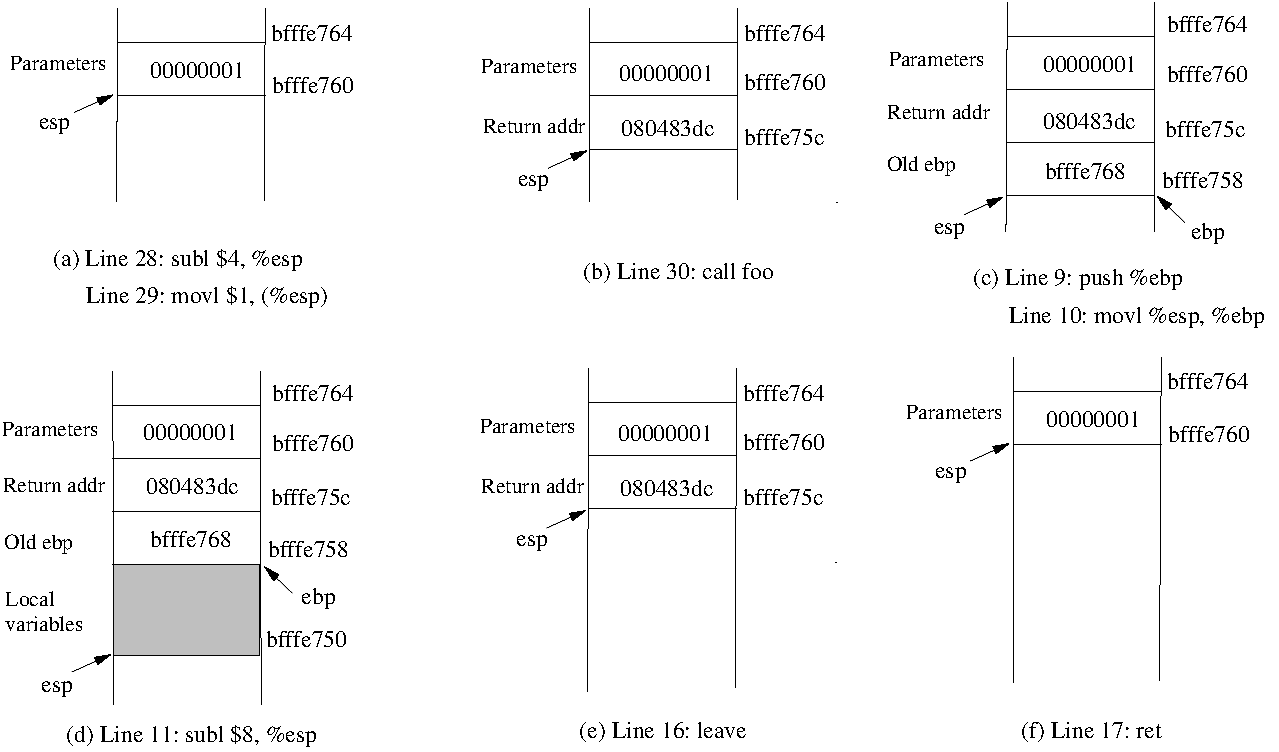
\includegraphics[width=0.95\textwidth]{\retFigs/enter_leave_foo.pdf}
	\caption{Entering and Leaving {\tt foo()}}
	\label{fig:enter_leave_foo}
\end{figure}


\begin{itemize}
\item \textbf{Line 28-29:}:
These two statements push the value $1$, i.e. the argument to the {\tt foo()}, 
into the stack. This operation increments {\tt \%esp} by four. The stack
after these two statements is depicted in Figure~\ref{fig:enter_leave_foo}(a).

\item \textbf{Line 30: \texttt{call foo}}: 
The statement pushes the address of the next instruction that 
immediately follows the {\tt call} statement into the 
stack (i.e the return address), and then jumps to the 
code of {\tt foo()}. 
The current stack is depicted in Figure~\ref{fig:enter_leave_foo}(b).

\item \textbf{Line 9-10}:
The first line of the function {\tt foo()} pushes {\tt \%ebp} into
the stack, to save the previous frame pointer. The second
line lets {\tt \%ebp} point to the current frame. The current stack 
is depicted in Figure~\ref{fig:enter_leave_foo}(c). 

\item \textbf{Line 11: \texttt{subl \$8, \%esp}}:
The stack pointer is modified to allocate space (8 bytes) for 
local variables and the two arguments passed to {\tt printf}. 
Since there is no local variable in function {\tt foo}, the
8 bytes are for arguments only. 
See Figure~\ref{fig:enter_leave_foo}(d). 

\end{itemize}


\subsection{Leaving {\tt foo()}}

Now the control has passed to the function {\tt foo()}. Let us see what happens
to the stack when the function returns.

\begin{itemize}
\item \textbf{Line 16: \texttt{leave}}: This
instruction implicitly performs two instructions (it was a macro
in earlier x86 releases, but was made into an instruction later):
\begin{verbatim}
    mov  %ebp, %esp
    pop  %ebp
\end{verbatim}
The first statement releases the stack space allocated for the function; 
the second statement recovers the previous frame pointer. 
The current stack is depicted in Figure~\ref{fig:enter_leave_foo}(e). 

\item \textbf{Line 17: \texttt{ret}}: This instruction simply pops the return 
address out of the stack, and then jump to the return address.
The current stack is depicted in Figure~\ref{fig:enter_leave_foo}(f).

\item \textbf{Line 32: \texttt{addl \$4, \%esp}}: Further restore the stack by
releasing more memories allocated for {\tt foo}. 
As you can see that the stack is now in exactly the same state as it was
before entering the function {\tt foo} (i.e., before line 28). 
\end{itemize}



% *******************************************
% SECTION
% *******************************************
\section{Informe de Laboratorio}

%%%%%%%%%%%%%%%%%%%%%%%%%%%%%%%%%%%%%%%%

Debe enviar un informe de laboratorio detallado, con capturas de pantalla, para describir lo que ha hecho y lo que ha observado.
También debe proporcionar una explicación a las observaciones que sean interesantes o sorprendentes.
Enumere también los fragmentos de código más importantes seguidos de una explicación. No recibirán créditos aquellos fragmentos de códigos que no sean explicados.
%%%%%%%%%%%%%%%%%%%%%%%%%%%%%%%%%%%%%%%%


% *******************************************
% SECTION
% *******************************************
\section*{Agradecimientos}

Este documento ha sido traducido al Español por Facundo Fontana



\end{document}

